\chapter{Introduction}
%\paragraph{Scheduling on a high level}
Computer systems need resources to function. 
Often times these reources are finite and scarce. 
Scheduling can be viewed as a governance model that \textit{governs} how the resources are shared among users and how various parts of the system function together. 
The governance model is designed so as to meet goals about resource management and performance of the system. 
As an example, an operating system uses resources such as memory, CPUs, and disk.
It allows multiple processes to use these resources at the same time. 

%\paragraph{Scheduling's history}
Scheduling is a well studied problem both from theoretical and practical perspectives. 
Typically a scheduling problems is tasked with an objective and with a goal to find a schedule that can either meet the objective or get close to it.
Many scheduling problems are difficult to solve (NP hard).
\todo{For example, job scheduling with deadline}.
There are a variety of techniques to solve scheduling problems such as heuristics, dynamic programming or greedy algorithms. 

%\paragraph{Scheduling for databases}
In this dissertation, we study the problem of scheduling for modern database systems.
We distinguish traditional database systems and modern database systems based on three aspects which are closely related to the scheduling problem: modern hardware, data volumes, and deployment environments.
We discuss these aspects below and explain how they are related to the scheduling problem. 

Over the past few years hardware has steadily evolved. 
Modern hardware includes large main memories, Non-Uniform Memory Access (NUMA) patterns and large number of CPU cores.
%To leverage the capabilities of the modern hardware comprehensively, database architecture needs a fundamental shift from its traditional roots. 
Traditional database architecture comes from a time when memories were smaller, data were mostly resident on disks and multi-core parallelism was uncommon. 
Therefore in contrast to traditional databases, modern databases have two resources in abundance: CPU parallelism and memory.
Scheduling involves managing resources, therefore there is a place for schedulers in modern database architecture. 

Next we look at data volume aspect.
Big data means that we are generating tremendous amount of data.
To process the large amount of data efficiently, data processing engines have to leverage all the hardware features effectively. 
However, we are experiencing a growing \textit{deficit} between the pace of hardware performance improvements and the pace that is demanded of data processing kernels to keep up with the growth in data volumes.

\begin{figure}
	\centering
	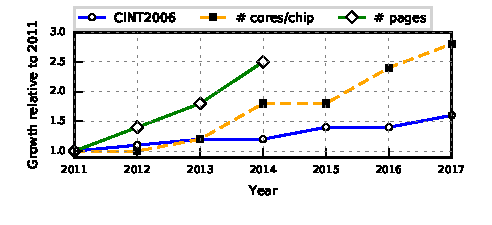
\includegraphics[width=\columnwidth]{system/figures/deficit.pdf}
%	\vspace*{-2em}
	\caption{\textbf{Processor performance improvement as measured by the highest reported CINT2006 benchmark result for Intel Xeon chips from~\cite{cpu2006} compared to the number of pages indexed by Google (using estimates made by~\cite{google-pages-db}). The figure does not show the increase in the number of queries (which is about 2.5X for Google search queries from 2011--14), and the increase in the complexity of queries as applications request richer analytics. These aspects make the deficit problem worse. The figure also shows the maximum number of cores per chip used in reported CINT2006 results over time. Interestingly (and not shown in the figure), both the minimum and the average amount of memory per chip in the reported CINT2006 results has grown by $\approx$4X from 2011 to 2017.}}
	% For example, the number of Google search queries has gone up by a factor of 6X in the time period shown in the graph above.}
	\label{fig-deficit}
\end{figure}

Figure~\ref{fig-deficit} illustrates this deficit issue by comparing improvements in processor performance (blue line) with the growth rate of data (green line), using the number of pages indexed by Google as an illustrative example. This data growth rate is conservative for many organizations, which tend to see a far higher rate of increase in the data volume; for example, Facebook's warehouse grew by 3X in 2014~\cite{fb-growth-14}. This figure also shows (using a dotted orange line with squares) the growth in the number of cores per processor over time. As one can observe, the number of cores per processor is rising rapidly. % as multi-core parallelism is critical for processor vendors.
%to realizing overall higher processor performance.
%(While we do not consider this further in this paper, the number of cores per processing unit is even higher for non-traditional processors/co-processors.)
% Thus, the demands on query processing can't simply be met by only throwing more chips/processors at the problem.
%Thus, there is a critical need for systems that can exploit the full potential of the hardware parallelism that is available in each box.
In addition, %as noted in the caption of the figure,
since 2011 the main memory sizes are also growing rapidly, and there is an increasing shift to larger main memory configurations. Thus, there is a critical need for in-memory data processing methods that \textit{scale-up} to exploit the full (parallel) processing power that is locked in commodity multi-core servers today.
\todo{Explain how growing data volume relates with scheduling}

Third, we look at deployment environments. 
The most common deployment method few years ago was "on-premise database", which means an enterprise would host the database software on a local machine(s) . 
Today cloud databases have changed how databases are deployed.
Cloud providers host and manage databases on their cloud platforms. 
The cloud provider takes care of concerns such as elasticity, fault tolerance, and replication.
The database engine may be hosted on a number of hardware platforms or virtualized environments in the cloud.
Irrespective of the host environment, the database is still expected to offer the best performance and meet the Service Layer Objectives (SLO) promised to the client of the database service. 
\todo{Explain how cloud databases relates with scheduling}